\immediate\write18{makeindex manual}
\immediate\write18{makeglossaries manual}
\documentclass{article}
\usepackage{authblk}
\usepackage{changes}
\usepackage[nonewpage]{imakeidx}
\usepackage{amsmath}
\usepackage{mathrsfs}
\usepackage{amsfonts}
\usepackage{hyperref}
\usepackage{lscape}
\usepackage{upgreek}
\usepackage[acronym]{glossaries}
\usepackage{tikz}
\tikzset{
	treenode/.style = {shape=rectangle, rounded corners,
		draw, align=center,
		top color=white, bottom color=blue!20},
	exp/.style     = {treenode, font=\Large, bottom color=orange!30},
	data/.style     = {treenode, font=\Large, bottom color=red!30},
	sample/.style      = {treenode, font=\Large,bottom color=blue!30},
	fit/.style      = {treenode, font=\Large,bottom color=green!30},
	entry/.style      = {treenode, font=\Large,bottom color=white}
}
%%%%%%%%%%%%% new commands
\newcommand{\code}[1]{\mbox{\textcolor{red!90}{#1}}}
\newcommand{\file}[1]{\mbox{\textcolor{green}{#1}}}
\newcommand{\argument}[1]{\mbox{\textcolor{cyan}{#1}}}
\newcommand{\function}[1]{\mbox{\textcolor{orange}{#1}}}
\newcommand{\PyQENS}{{\it\bf PyQENS}}
%%%%%%%%%%%%%%%%%%%%%%%% title information
\author[1,2]{Christian Beck\thanks{ORCID: \href{https://orcid.org/0000-0001-7214-3447}{0000-0001-7214-3447}; mail: \href{mailto:christian.beck@uni-tuebingen.de}{christian.beck@uni-tuebingen.de}}}
\affil[1]{Institut f\"ur Angewandte Physik, Universit\"at T\"ubingen,  Auf der Morgenstelle 10, 72076 T\"ubingen, Germany}
\affil[2]{Institut Max von Laue - Paul Langevin, 71 avenue des Martyrs, 38042 Grenoble, France}

\title{\PyQENS\\A python toolbox for fitting QENS Data}
%%%%%%%%%%%%%other stuff
\makeindex[title=\,] % for index
\makeglossaries % for glossary
\newacronym{qens}{QENS}{quasielastic neutron scattering}
\newacronym{nbs}{NBS}{neutron back-scattering}
\newacronym{fws}{FWS}{fixed window scan}
\newacronym{ifws}{IFWS}{inelastic fixed window scan}
\newacronym{efws}{EFWS}{elastic fixed window scan}
\newacronym{tof}{TOF}{time of flight}
\newacronym{fwhm}{FWHM}{full width at half maximum}
\newacronym{eisf}{EISF}{elastic incoherent structure factor}
\begin{document}
	\maketitle
	\newpage
	\tableofcontents
	\section{Introduction}
This document is a manual for the python routines called \PyQENS. The routines are mend for analyzing \gls{qens} spectra of samples containing diffusive processes such as protein samples (powders, solutions), as well as colloidal suspensions, etc.

The software is written in such a way, that it can treat spectra from different instruments including \gls{nbs} as well as \gls{tof} measurements. It can also treat \gls{fws} with several analysis methods or can include these measurements in the analysis of the full \gls{qens} spectra to improve the fits.

\section{Software Requirements}
\label{Software}
The \PyQENS\, routines are written for Python\,3. Some parts of the routines are based on Mantid \cite{Arnold2014}. To have full functionality of the routines, it is necessary, that the Python version matches the one of Mantid. It should also be possible to run the scripts in the Mantid-workbench \added{To be tested!!}. The main part of the scripts is however thought as standalone and can be run without a Mantid installations.
\section{A general comment on fit complexity}
\label{CommentFitparameters}
The routines of \PyQENS\, use fits in two different ways. The first type of fits use an excess of fit parameters to obtain a description of the data set which matches as good as possible. This can be used in the case of the resolution function (see Section \ref{FIT:VANADIUM}) \cite{Grimaldo_2015_JPhysChemLett} or might also be applied in the case of the solvent. These parameters might have big uncertainties and are normally not linked directly to physical meaningful parameters. However, since the whole parameter set is fixed to these constants in later fits, an accurate description can result in improved fit results at the end.


	\section{TODO}
savepath manual
binning


	\section{The main script}
\subsection{The Protocol}
\label{Main:Protocol}
	\section{Experiment Class}
\begin{figure}
	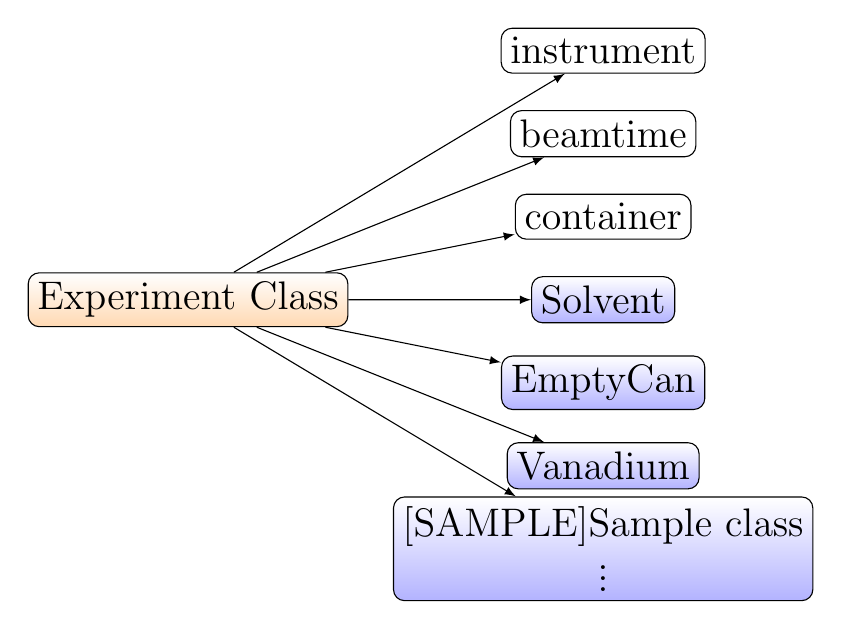
\begin{tikzpicture}
	[
	grow                    = right,
	sibling distance        = 3em,
	level distance          = 15em,
	edge from parent/.style = {draw, -latex},
	every node/.style       = {font=\footnotesize},
	sloped
	]
	\node [exp] {Experiment Class}
	child { node [sample] {\hyperref[SAMPLE]{Sample class}\\\vdots}}
	child{node[sample]{Vanadium}}
	child{node[sample]{EmptyCan}}
	child{node[sample]{Solvent}}
	child{node[entry]{container}}
	child{node[entry]{beamtime}}
	child{node[entry]{instrument}}
	;
	\end{tikzpicture}
	\caption{Graphical overview of the structure of the Experiment class}
	\label{Pic:Experiment:Overview}
\end{figure}

	\section{Sample Class}
\begin{figure}
	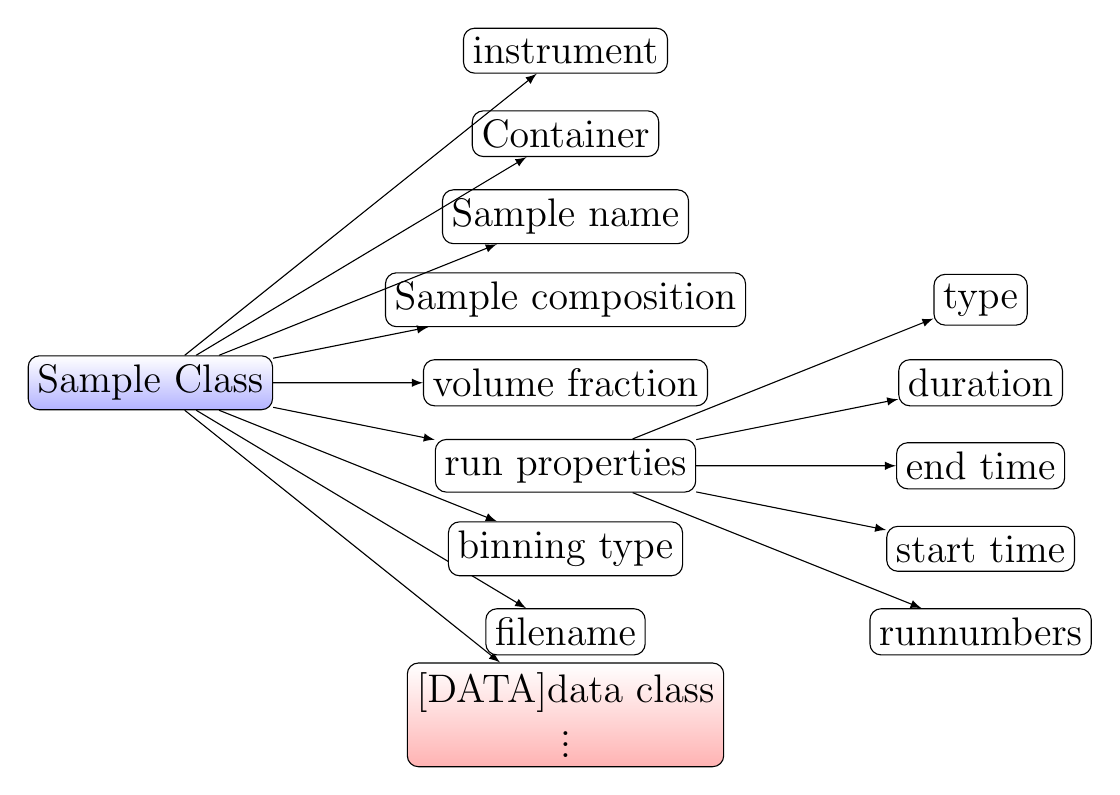
\begin{tikzpicture}
	[
	grow                    = right,
	sibling distance        = 3em,
	level distance          = 15em,
	edge from parent/.style = {draw, -latex},
	every node/.style       = {font=\footnotesize},
	sloped
	]
	\node [sample] {Sample Class}
	child { node [data] {\hyperref[DATA]{data class}\\\vdots}}
	child { node [entry] {filename}}
	child { node [entry] {binning type}}
	child{node [entry] {run properties}
		child { node [entry] {runnumbers}}
		child { node [entry] {start time}}
		child { node [entry] {end time}}
		child { node [entry] {duration}}
		child { node [entry] {type}}
	}
	child { node [entry] {volume fraction}}
	child { node [entry] {Sample composition}}
	child { node [entry] {Sample name}}
	child { node [entry] {Container}}
	child { node [entry] {instrument}}
	;
	\end{tikzpicture}
	\caption{Graphical overview of the structure of the sample class}
	\label{Pic:SAMPLE:Overview}
\end{figure}

	\section{Data Class}
\label{DATA}
\begin{figure}
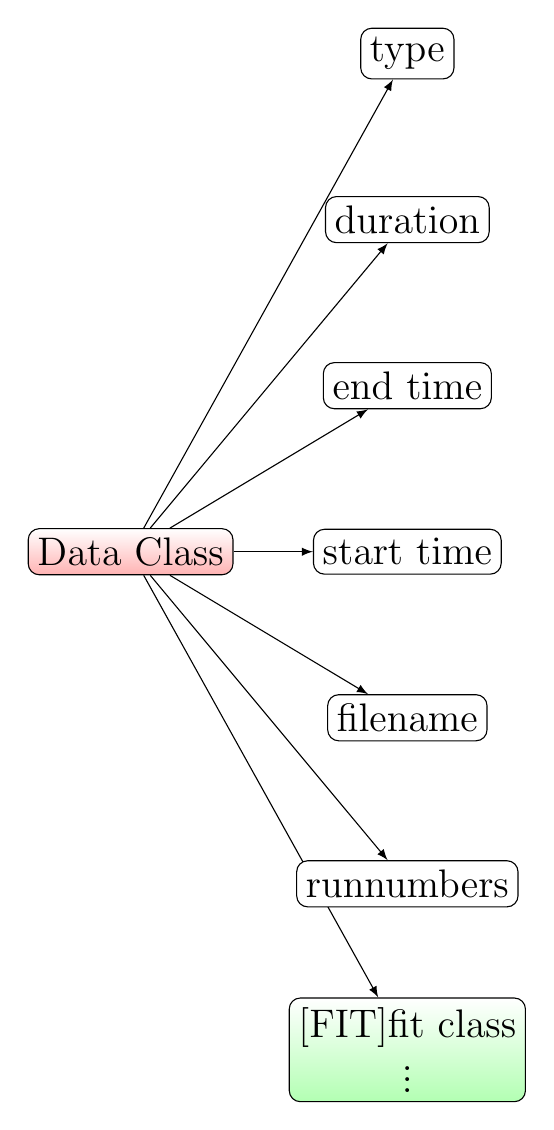
\begin{tikzpicture}
[
grow                    = right,
sibling distance        = 6em,
level distance          = 10em,
edge from parent/.style = {draw, -latex},
every node/.style       = {font=\footnotesize},
sloped
]
\node [data] {Data Class}
child { node [fit] {\hyperref[FIT]{fit class}\\\vdots}}
child { node [entry] {runnumbers}}
child { node [entry] {filename}}
child { node [entry] {start time}}
child { node [entry] {end time}}
child { node [entry] {duration}}
child { node [entry] {type}}
;
\end{tikzpicture}
\caption{Graphical overview of the structure of the data class}
\label{Pic:DATA:Overview}
\end{figure}
	\section{The Fit Class}
\label{FIT}
\subsection{The Resolution function}
\label{FIT:VANADIUM}
\index{Vanadium|see {Resolution}}
\index{Resolution}
Normally, one is interested in describing the resolution function of the instrument as accurate as possible. Since in most of the cases, an accurate physical description describing all of the features of the instrumental resolution function is missing, an adapted parametrization is often chosen. See also Section \ref{CommentFitparameters}. 
In the routines of \PyQENS, the resolution function can be fitted with a combination of 
\begin{itemize}
	\item Gaussian functions (\code{VanadiumData.NumberOfGaussians=i}),
	\item Lorentzian functions (\code{VanadiumData.NumberOfLorentzians=j}) as well as
	\item Voigt functions (\code{VanadiumData.NumberOfVoigts=k})
\end{itemize} with \code{i,j,k} being integers. The widths and scalings are set to be positive values. The center is free and can shift. By doing so, also asymmetric resolution functions can be treated \cite{Grimaldo_2015_JPhysChemLett}. 
It can also include flat or sloped backgrounds (\code{VanadiumData.bkg="slope/flat/none"}).
\subsection{The Fit levels for QENS spectra}
\label{FIT:LEVEL} The routines of \PyQENS\, are able to treat different types of fits. What type of fits are performed depends on the data as well as on the fit model. 
For \gls{qens} data, the routines recognize on the given fit model, what fit-level should be applied. 
\begin{enumerate}
	\item As a first step, fits performed for each $q$ individually are recommended (Fitlevel $q$\index{Fitlevel!q|textbf}).
	\item As a second step, fits including the $q$ dependence can performed. These fits, fitting each sample individually (Fitlevel S)\index{Fitlevel!S|textbf}, can include $q$-independent parameters such as \textit{e.g.} fraction of immobile particles in the sample \cite{Beck_2019_CrystGrowthDes}.
	\item As a last step, fits can be performed, which take several \gls{qens} spectra of one Experiment (Fitlevel E) \index{Fitlevel!E|textbf} into account. By doing so, fits determining parameters, which are independent from the control parameters (\textit{e.g.} time, pressure, temperature, \dots) can be determined. In addition, this fit approach can be used to analyzed kinetically changing samples which were investigated by \gls{fws}.
\end{enumerate}
\subsection{The different implemented fit models}
	A set of different fit models is implemented for the analysis of the \gls{qens} spectra. Here, the flags to use them as well as the model functions and main references are reported. An overview of different applications can be found \textit{e.g.} in \cite{Grimaldo_2019_QuartRevBiophys}. In case, other fit models are desired, they can be written manually in the file \file{fitfunctions.py} by respecting the corresponding syntax or the function \file{addfitfunction.py}\added{to be written!} can be use to add the fit model via an graphical interface. If a data set is fitted several times, the results are save in a list of Fit Classes. To perform fits, the function \function{Fit.QENS} is called with the data set as well as with the corresponding \argument{fit name}:
\begin{enumerate}
	\item \argument{Vanadium}: \index{Vanadium}\index{Resolution!Fit} This should be used to fit the resolution function of the instrument. The fit function is assembled based on the parameters set as described in Section \ref{FIT:VANADIUM}.
	\item \argument{D2O}:
	\index{Solvent}\index{D$_2$O} 
	This fit used the \gls{fwhm}\added{check!!!} of IN6\added{check!!!} measurements to fix the width of the solvent (D$_2$O). It is fitted for each $q$ independently to determine the absolute values. See also Point \ref{FIT:SOLVENT:D2Ofixed} in Section \ref{FIT:SOLVENT:MODEL}.
	\item \argument{SolventOneLorentz}\index{Solvent}:
	\item \argument{SolventTwoLorentz}\index{Solvent}: 
	\item \argument{twolorentz\_free\_q}\index{Fitmodel}: This model fits the data on each $q$ independently\index{Fitlevel!q}:
	\begin{equation}
	S(q,\omega)=A_0(q)\mathscr{L}_\gamma(\omega)+(1-A_0(q))\mathscr{L}_{\gamma+\Gamma}(\omega)\label{eq:FIT:standardmodel}
	\end{equation}
	with $A_0$ being the \gls{eisf}. In a second step, the $q$-dependence of the \gls{eisf} \cite{Grimaldo_2015_PhysChemChemPhys} as well as the one from $\gamma$ and $\Gamma$ \cite{Beck_2018_JPhysChemB} are fitted with the following functions:
	\begin{eqnarray}
	A_0&=&p+(1-p)\exp\left(-\frac{q^2a^2}{5}\right)\cdot\notag\\&&\cdot\left[s\left|\frac{3j_1(qR)}{qR}\right|^2+(1-s)\frac{1+2j_0(qa_m)}{3}\right]\\
	\gamma&=&Dq^2\label{eq:FIT:brown}\\
	\Gamma&=&\frac{D_{int}q^2}{1+D_{int}\tau}\label{eq:FIT:jump}
	\end{eqnarray}
	\item \argument{brownian\_diffusion\_internal\_free}: This model uses Equation \ref{eq:FIT:standardmodel} implying the $q$ dependence of of Equation \ref{eq:FIT:brown}. The \gls{eisf} as well as $\Gamma$ is kept as $q$-dependent parameter. The fits are performed as sample dependent fits. \index{Fitlevel!S}
	\item \argument{jump\_diffision\_internal\_jump}: This model uses Equation \ref{eq:FIT:standardmodel} implying the $q$ dependence of of Equation \ref{eq:FIT:jump} both for the internal as well as for the global diffusion. The \gls{eisf} is kept as $q$-dependent parameter. The fits are performed as sample dependent fits. \index{Fitlevel!S}
	\item \argument{immobile\_jump\_diffusion\_internal\_jump}: This model describes the scattering function assuming a certain fraction of immobile scatterers:
		\begin{eqnarray}
		S(q,\omega)&=&A_c\cdot D(q) +(1-A_c)(A_0(q)\mathscr{L}_\gamma(\omega))+\notag\\
		&&Ac(1-A_0(q))\mathscr{L}_{\Gamma}(\omega)+(1-A_c)(1-A_0(q))\mathscr{L}_{\gamma+\Gamma}(\omega)\label{eq:FIT:crystalmodel}
		\end{eqnarray}
	The internal as well as the global diffusion implies the $q$ dependence of Equation \ref{eq:FIT:jump}. The \gls{eisf} is kept as $q$-dependent parameter. The fits are performed as sample dependent fits. \index{Fitlevel!S} \cite{Beck_2019_CrystGrowthDes}
	\item \argument{brownian\_diffusion\_internal\_jump}: This model uses Equation \ref{eq:FIT:standardmodel} implying the $q$ dependence of of Equation \ref{eq:FIT:brown} and Equation \ref{eq:FIT:jump}. The \gls{eisf} is kept as $q$-dependent parameter. The fits are performed as sample dependent fits. \index{Fitlevel!S}
	\item \argument{brownian\_diffusion\_internal\_switching}: This model fits the data on the Fitlevel S\index{Fitlevel!S}. The global diffusion is described by a Brownian diffusion with $\gamma=D\cdot q^2$. The internal diffusion is described by Grimaldo \textit{et.al.} \cite{Grimaldo_2015_PhysChemChemPhys}. The theoretical framework is given by Roosen-Runge \textit{et al.} \cite{Roosen-Runge2016}. It is described by two linked Lorentzian functions:
	\begin{eqnarray}
		\Gamma_{1,2}&=&D_{1,2}\cdot q^2\\
		\Lambda&=&\sqrt{\left(\Gamma_1-\Gamma_2+\frac{1}{\tau_1}-\frac{1}{\tau_2}\right)^2+\frac{4}{\tau_1\tau_2}}\\
		\lambda_{1,2}&=&\frac{\Gamma_1+\Gamma_2+\frac{1}{\tau_1}+\frac{1}{\tau_2}\pm\Lambda}{2}\\
		\alpha&=&\frac{\Lambda}{\tau_1+\tau_2}\left((\tau_1+\tau_2)\lambda_1-\tau_1\Gamma_2-\frac{\tau_1}{\tau_2}-\tau_2\Gamma_1-\frac{\tau_2}{\tau_1}-2\right)\\
		S_{int}(q,\omega)&=&\alpha\mathscr{L}_{\lambda_1}(\omega)+(1-\alpha)\mathscr{L}_{\lambda_2}(\omega)
	\end{eqnarray}	
\end{enumerate}	
\subsection{Solvent handling}
\index{Solvent}
\subsubsection{Solvent treatment}
\label{FIT:SOLVENT}\index{Solvent!treatment}
Two different methods exist to treat the solvent contribution in QENS spectra:
\begin{enumerate}
	\item \label{FIT:SOLVENT:Solventsubtract}{\bf Subtraction of the solvent contribution:} The solvent contribution can be subtracted from each QENS spectra. In this case, the remaining signal is given by the scattering function of the dissolved particles. To subtract the solvent contribution, set the flag \code{solventtreatment='subtractsolvent'}. 
	\item \label{FIT:SOLVENT:Solventmodel}{\bf modeling the solvent contribution: } Next to subtracting the solvent contribution, it can be taken into account in the fit model. To do so, the the flag has to be set to \code{solventtreatment='modelsolvent'}
\end{enumerate}
\subsubsection{Solvent rescaling}
\index{Solvent!rescaling}
\label{FIT:SOLVENT:RESCALE}
In both cases mentioned above in section \ref{FIT:SOLVENT}, the solvent contribution measured from the pure solvent has to be rescaled accordingly to the volume fraction: 
\begin{enumerate}
	\item If the volume fraction is known, it can be fixed. for a certain list of proteins (\added{todo}) the volume fraction is calculated based on the concentration. If this is not desired, the volume fraction can be specified in the Protocol (see Section \ref{Main:Protocol}) as optional parameter. This method is enabled by choosing \code{solventscaling='fix'}.
	\item If the volume fraction is not known, this parameter can be set as fit parameter in the fit. It is recommended to set this parameter constant in $q$\index{Fitlevel!q}, \textit{i.e.} use at least Fitlevel $S$ \index{Fitlevel!S} or Fitlevel $E$ \index{Fitlevel!E}. However, it is possible to use these three options:
	\begin{itemize}
		\item \code{solventscaling='freeq'}
		\item \code{solventscaling='freeS'} (recommended)
		\item \code{solventscaling='freeE'} (recommended)
	\end{itemize}
	For a more detailed description of the fit levels\index{Fitlevel}, see Section \ref{FIT:LEVEL}.
\end{enumerate}
\added{To be written}
\subsubsection{Solvent modeling}
\label{FIT:SOLVENT:MODEL}\index{Solvent!modeling}
For both cases mentioned in Section \ref{FIT:SOLVENT}, subtraction of the solvent or its modeling, there are several methods, how the solvent data is treated. These are listed in the following:

\begin{enumerate}
	\item \textbf{Use experimental data:}\label{FIT:SOLVENT:direct} In this option, a measured data set is used to treat the solvent in the spectra. To use this option, the flag \code{solventmodel='direct'} has to be chosen.\\
	\textit{Warning:} In combination with \code{solventtreatment='modelsolvent'} the fit results might look fuzzy, if the solvent was measured not with good statistics.
	\item \label{FIT:SOLVENT:D2Ofixed}{\bf D2O treatment:} In this method, the water contribution is fitted with one Lorentzian function whose temperature and $q$-dependent width is fixed based on \gls{tof} data as described by Grimaldo \textit{et al.} \cite{Grimaldo_2015_EPJWebofConferences}. This option is used with \code{solventmodel='D2Ofixed'}.
	\item \label{FIT:SOLVENT:onelorentz}\textbf{Model solvent contribution with \textit{one} Lorentzian function:} This option uses one free Lorentzian function (free width and free scaling) to model the contribution of the solvent. To use this model, set \code{solventmodel='onelorentz'}.
	\item \label{FIT:SOLVENT:twolorentz}\textbf{Model solvent contribution with \textit{two} Lorentzian functions:} This option uses one free Lorentzian function (free widths and free scaling parameters) to model the contribution of the solvent. To use this model, set \code{solventmodel='twolorentz'}.
\end{enumerate}
Option \ref{FIT:SOLVENT:twolorentz} should only be used if there is a significant contribution of the solvent visible in the investigated energy transfer window. broad energy resolutions or limited energy transfers might hide contributions and might therefore allow to use simplified models. See also Section \ref{CommentFitparameters}.
	\section{Plot and saving options}
There are several plot and saving options. The different options can be combined if they are handed in as a list.
\begin{itemize}
	\item \code{plotresults='fits'}: This option displays the fits. Fits of \Gls{qens} are displayed with $\hbar\omega$ as abscissa, while \gls{fws} are displayed with $q$ as abscissa. The ordinate in both cases is in logarithmic scale. In case \gls{fws} and \gls{qens} are combined, they are displayed similar to the pure \gls{qens} spectra. the \gls{fws} are plotted also in the plots. 
	\item \code{plotresults='results'}: This option displays only the fit results but not the Fits itself.
	\item \code{plotresults='all'}: This option combines both options of \code{plotresults='fits'} and \code{plotresults='results'}.
	\item \code{plotresults='silent'}: These option generates the same figures as \code{plotresults='all'} but they are not displayed but only saved.
	\item \code{plotresults='none'}: This option does not create any figures.
	\item \code{plotresults='writeascii'}: This option saves all fit results as ascii, which might be usefull, if they should be treated later with other programs.
\end{itemize}
Next to plotting the fit results as explained above, a summary can be generated by activating the option \code{writesummary='all/fit/results/none'}. The options \code{writesummary='all/fit/results'} overwrites the option \code{plotresults='none'} to \code{plotresults='all/fit/results'}.

Files are saved as default as ".eps" files. To change this can be saved by setting the flag \code{pictureextension} from \code{pictureextension='eps'} to \code{pictureextension='png'}
	\appendix
\section*{Appendix}
\addcontentsline{toc}{section}{Appendix}
\begin{landscape}
	\section{Overview of flags to control script}
	
\end{landscape}
\section{Index}
\printindex
\vspace{2cm}
\section{Glossary}\renewcommand*\acronymname{}
\printglossaries
\section{Literature}
\bibliographystyle{plain}
\bibliography{literature}
\end{document}